% =====================================================================
%  Part II (v3) --- learner-free RL paper, for TMLR. ANONYMIZED (double-blind).
%  THESIS (reframed, 2026-10-17 after discrimination experiments + referee review):
%  The reinforcement learning is at the level of the PROBLEM SOLVED and the
%  OUTCOME REACHED, NOT in the micro-dynamics. A self-organizing swarm
%  SOLVES the explore/exploit problem --- balances exploration and exploitation
%  and converges to the optimal allocation (ideal free distribution) --- with no
%  learner, no trained parameters, and (shown directly) NO reward signal in the
%  dynamics. We do NOT claim the micro-rule is a replicator / reward-proportional
%  update (it is not: recruitment is crowd-driven, the swarm is payoff-blind).
%  v2 claimed that and it was withdrawn (see REFEREE_REVIEW_2026-10-17.md,
%  DISCRIM_RESULTS.md). The experiments support: reaches the optimum; reward-free;
%  solves-but-does-not-learn (plateau + re-track); not a general learner (MARL).
%  At camera-ready restore author/affiliation, code/data URL, patent CoI, real
%  Part I citation; add permission line to reproduced Figs 1-2 if Part I is published.
% =====================================================================
\documentclass{article}
\usepackage{tmlr}      % submission = anonymized/double-blind; use [accepted] for camera-ready
\usepackage{amsmath,amssymb}
\usepackage{graphicx}
\graphicspath{{figures/}}
\usepackage{float}
\usepackage{xcolor}
\usepackage[colorlinks=true,linkcolor=blue!50!black,citecolor=blue!50!black,
            urlcolor=blue!50!black]{hyperref}

\title{Self-organizing reinforcement learning: a swarm approaches the explore--exploit optimum}
% Camera-ready author (restore at acceptance):
%   \author{\name Galen J. Wilkerson \email gwilkerson@komplexai.io \\ \addr Komplexity AI LLC}
\author{}

\begin{document}
\maketitle

\begin{abstract}
The explore/exploit trade-off is the core problem of reinforcement learning (RL). We show that a minimal
foraging swarm \emph{approaches the optimum}---the ideal-free / Nash-equilibrium allocation of the multi-agent
sharing game (an equilibrium, not a return maximum)---with no learner and no reward signal: self-organization
does the work. Agents explore by heavy-tailed (L\'evy) flights, recruit
neighbours to a discovery through a threshold cascade on their proximity network, and disperse again as a patch
crowds. This cascade cycle automatically balances exploration against exploitation and drives the collective
toward the optimal allocation of foragers across patches---the \emph{ideal free distribution} (foragers in
proportion to richness; the Nash equilibrium of the habitat-sharing game). We are careful about what
``reaches'' means: the swarm attains the \emph{shape} of this optimum (committed foragers track richness with
slope $0.94$) but not its exact equilibrium---it remains measurably exploitable. Because resource is shared,
total intake is the same for any interior allocation, so the optimum is a load-balancing \emph{equilibrium},
not a total-harvest maximum; the harvesting-efficiency side of foraging is analysed in the companion
paper~\citep{partI}. The matching is reached dynamically (within ${\sim}150$ steps) and is produced by the
coupling of recruitment to movement: remove the coupling and it collapses (slope $0.94\!\to\!0.08$). We are
deliberate about \emph{where} the reinforcement learning lives: at the level of the \emph{problem} and the
\emph{allocation reached}, not in the micro-dynamics. No step of the rule evaluates payoff---recruitment
responds to a local crowd signal---so the mechanism is reward-free \emph{by construction}; because under
resource sharing that crowd signal is informationally tied to payoff, ``reward-free'' is a statement about the
implementation, not a claim that no payoff-equivalent information is used. The swarm also \emph{reaches} this
allocation without \emph{learning} it: its quality plateaus and re-settles after the resources move, with no
cumulative gain. Against a trained reinforcement-learning baseline the comparison is embodiment-dependent: in an \emph{easier,
disembodied} version of the game a learner reaches the optimum more precisely, but in the \emph{same embodied}
environment as the swarm---matched sensing, movement, and actions---the reward-free swarm reaches $55\%$ of a
validated oracle ceiling at zero training, ahead of an online decentralized learner's $34\%$ (the $1.67\times$
intake ratio), and stays ahead across a horizon$\times$nonstationarity sweep. Both stay far from the ceiling,
and the learner is limited by its local architecture, not its training budget, so closing the gap would need a
higher-capacity learner, not more training. We scope the claim to this one minimal setting and decentralized
learner class---it \emph{bounds} rather than settles the comparison---and read it not as beating reinforcement
learning but as evidence the mechanism is \emph{worth pursuing}: it approaches the optimum competitively,
without the learner's overhead. The result is a concrete demonstration that the self-organizing physics of a minimal swarm can carry
a collective close to the optimum reinforcement learning seeks, with none of reinforcement learning's
machinery. The companion paper~\citep{partI} develops the underlying mechanism.
\end{abstract}

% =====================================================================
\section{Introduction}
Reinforcement learning (RL) is the machine-learning account of the explore/exploit trade-off: a system must
\emph{explore} to discover where reward is and \emph{exploit} what it has found, and good behaviour is the
behaviour that balances the two and settles at the best available payoff~\citep{SuttonBarto2018}. A foraging
swarm faces exactly this problem. Patches of resource are options of unknown location and yield; the swarm must
search for them and converge on the good ones, with only local sensing and no central controller. Because many
foragers share each patch, a forager's best available payoff is congestion-limited---the most it can get given
where everyone else is---so the problem is multi-agent and its optimum is a collective \emph{allocation} (each
forager at its best available payoff: the ideal-free / Nash equilibrium), not a single best option. The natural
question is whether a swarm that forages well is, in effect, reaching the optimum of this
reinforcement-learning problem, and if so, what plays the part of the learner.

We answer: the swarm approaches the optimum---it attains the optimal allocation's \emph{shape}---and there is
no learner, and, more strongly, no reward signal inside the dynamics at all. A minimal
self-organizing mechanism---L\'evy exploration, threshold recruitment to discoveries, and
density-dependent dispersal---balances exploration and exploitation and converges toward the optimal allocation
of foragers across patches (reaching its shape, though it remains measurably exploitable; \S\ref{sec:solve},
\S\ref{sec:compare}). The point of this paper is a claim about \emph{level of
abstraction}. The reinforcement learning is at the level of the \emph{problem solved} and the \emph{outcome
reached}, not at the level of the micro-rule. We are explicit about this because a tempting reading---that the
recruitment rule is itself a reward-following learning update---is false, and we show it is false. The agents
never evaluate how good a patch is; recruitment responds to local crowding, not to payoff. What is remarkable
is precisely that a system with \emph{none} of reinforcement learning's machinery---no value function, no
policy parameters, no training, no reward signal---nonetheless lands near the optimum reinforcement learning is
built to find.

\paragraph{Claims.} The paper makes four claims, each stated so it can be checked against evidence.
\begin{enumerate}\setlength\itemsep{2pt}
  \item \textbf{(The swarm approaches the explore/exploit optimum.)} The self-organizing cascade cycle
        balances exploration and exploitation and converges to the \emph{shape} of the optimal foraging
        allocation---the ideal free distribution (matching slope $0.94$)---reached dynamically and caused by the
        recruitment--movement coupling (remove it and matching collapses to $0.08$); the exact equilibrium is
        not reached---the swarm stays measurably exploitable (\S\ref{sec:solve},~\S\ref{sec:compare}).
  \item \textbf{(Learner-free and reward-free.)} It does so with no value function, no policy parameters, and
        no training---and the dynamics contain no reward signal: the agents never read a payoff, and
        recruitment is driven by crowding, not by reward (\S\ref{sec:how}).
  \item \textbf{(It reaches the allocation, it does not learn.)} Reaching this allocation is not epistemic
        learning: the configuration's informativeness rises once and plateaus, and re-settles after the
        resources move with no cumulative gain (\S\ref{sec:how}).
  \item \textbf{(Competitive without the overhead.)} Matched for embodiment---same environment, sensing,
        movement, and actions---the reward-free swarm is competitive with, and here ahead of ($1.67\times$ the
        cumulative intake of), an online decentralized RL learner, at no training, reward signal, or parameters;
        a learner's apparent advantage appears only in an easier \emph{disembodied} version of the task
        (\S\ref{sec:compare}). It does not, however, transfer to a different reward structure---a fixed,
        reward-blind mechanism cannot.
\end{enumerate}

\paragraph{What is, and is not, claimed.} We claim that the \emph{optimum} of a reinforcement-learning
problem---the optimal explore/exploit allocation, the ideal-free / Nash equilibrium---is reached by a physical,
self-organizing mechanism with no learner. We do \emph{not} claim that the micro-dynamics are a
reinforcement-learning algorithm, a reward-following update, or the replicator equation: the recruitment rule
is reward-free \emph{by construction} (no step reads payoff; \S\ref{sec:mech},~\S\ref{sec:how}). We do
\emph{not} claim the optimum is a total-reward maximum---under resource sharing it is an equal-intake
equilibrium (App.~\ref{app:optimum}). And we do \emph{not} claim epistemic learning: the swarm reaches the
optimum, it does not improve an estimate from experience. Return genuinely varies---and the explore/exploit
stakes bite---only in the \emph{dynamic, embodied} setting (\S\ref{sec:compare}), where cumulative intake
differs across policies; that is where we compare to a learner. The content is both precise and, we think,
important: a system with \emph{none} of reinforcement learning's machinery lands exactly where learning-in-
games dynamics converge, and in the embodied setting forages competitively with a learner---and whether a
collective ``beats'' RL \emph{flips} with embodiment (\S\ref{sec:compare}), a caution for how such comparisons
are run.

\paragraph{Scope and the companion paper.} The swarm's mechanism---a spatial threshold recruitment cascade that
self-organizes to a critical ``cascade window''---is developed in a companion paper~\citep{partI}. We summarise
it (with figures) only as far as the present reading needs and keep the paper self-contained for a
machine-learning reader; the companion paper is provided, anonymized, as supplementary material so a reviewer
can check the mechanism's details directly---including the parameter sweeps (phase diagrams over connectivity
and activation threshold) that establish the self-organized ``cascade window,'' and the movement-neutrality of
recruitment, both of which we cite rather than re-derive here. Our claims concern the explore/exploit problem
and the allocation the swarm reaches.

% =====================================================================
\section{Related work}
\label{sec:related}
\paragraph{The explore/exploit problem and bandits.} The multi-armed bandit~\citep{robbins1952bandit,
lattimore2020bandit} is the canonical formalisation of explore/exploit, and the one-state reduction of the
general RL problem~\citep{SuttonBarto2018}. Our setting is its multi-agent, resource-sharing instance: arms are
patches whose per-capita yield falls as more foragers work them, so the optimum is an allocation, not a single
best arm.

\paragraph{The optimum: ideal free distribution and habitat games.} The optimal allocation of foragers over
patches is the \emph{ideal free distribution} (IFD): foragers distribute in proportion to resource so that
per-capita intake is equal and no forager gains by moving~\citep{fretwell1969ideal}. This is the Nash
equilibrium of the habitat-selection (congestion) game~\citep{rosenthal1973congestion,wardrop1952road} and the
standard optimality criterion in behavioural ecology. We use the IFD only to \emph{characterise the solution}
the swarm reaches; we do not claim the swarm reaches it by playing the game or by any game-solving procedure.

\paragraph{Learning in games as the mean field of RL.} Reward-proportional reinforcement is, in the
large-population mean field, the replicator equation~\citep{borgers1997learning}, the bridge used to analyse
multi-agent learning dynamically~\citep{hofbauer1998evolutionary,sandholm2010population,tuyls2005evolutionary,
bloembergen2015evolutionary}. This is the level at which one \emph{might} hope to identify a physical swarm
with RL. We deliberately do \emph{not} rest our claim there: \S\ref{sec:how} shows the swarm's micro-dynamics
are reward-free and are not a replicator update. Our identification is at the problem/solution level instead.

\paragraph{Swarm optimisation, stigmergy, and designed game-solvers.} Metaheuristics such as
particle-swarm~\citep{kennedy1995particle} and ant-colony optimisation~\citep{dorigo1996ant} coordinate many
simple units, but they are \emph{designed} to optimise a supplied objective and carry memory (a personal/global
best; a pheromone table). Stigmergic foraging is usually read as \emph{reinforcement}, with the pheromone field
an external memory / value estimate~\citep{vellinger2025pheromones}. Decentralised multi-agent control reaches
Nash / potential-game equilibria from local information \emph{by design}~\citep{marden2009cooperative}, and
bee-inspired allocation reaches a Nash, optimal allocation by designed local rules~\citep{quijano2010honeybee}.
Ours is none of these: it is not a designed optimiser, it carries no memory or value estimate, and it uses no
reward---it is a physical mechanism whose self-organized dynamics happen to settle at the problem's optimum.
That contrast makes the claim precise: the swarm is the memory-free, reward-free limit these methods are not.

\paragraph{Minimally intelligent agents reaching an optimum.} That non-optimising agents can reach a market's
competitive allocation is the ``zero-intelligence'' result of experimental economics~\citep{gode1993allocative}.
Our result is in this spirit---the structure of the interaction, not the sophistication of the agent, does the
optimising---extended to a spatial, self-organizing foraging swarm and to the explore/exploit problem.
Reaching an equilibrium without computing payoffs also connects to no-regret and evolutionary learning
dynamics, which provably converge to equilibria of the underlying
game~\citep{sandholm2010population,hofbauer1998evolutionary}; our mechanism is the limiting case that uses no
regret signal and no payoff at all.
We make no entropy-regularised (``soft'') RL claim~\citep{haarnoja2018soft,ziebart2008maxent}: the spread of
the converged allocation is the ideal free distribution set by resource sharing, not a temperature.

% =====================================================================
\section{The physical model: a self-organizing forager}
\label{sec:mech}
The full model, its critical ``cascade window,'' and the efficiency analysis are in the companion
paper~\citep{partI}; here is what the present reading needs, drawn in Figs.~\ref{fig:mech} and~\ref{fig:cycle}.
$N$ foragers move on a torus. An inactive agent \emph{explores} by heavy-tailed (L\'evy) hops. An agent that
lands on resource becomes \emph{active} (a \emph{seed}) and \emph{recruits} its neighbours: recruitment is a
linear-threshold cascade on the proximity graph (an edge joins agents within sensing range $r$). An agent
activates when the active fraction of its neighbours crosses a threshold, $a/k\ge\phi$ ($a$ active neighbours,
$k$ neighbours), and recruited agents switch to short local moves toward the find. Because activation is
\emph{degree-normalized}, the same rule that spreads a cascade also stifles it once a neighbourhood crowds and
$a/k$ falls back below $\phi$: recruitment to a crowded patch shuts off. So the swarm aggregates on a find and
then releases to explore again. Crucially for what follows, \textbf{no step of this rule reads a payoff}: a
seed fires on \emph{contact} with resource, and recruitment responds to the \emph{active fraction} of
neighbours---a crowd signal---never to how rich a patch is or how much intake an agent receives.

\begin{figure}[t]\centering
  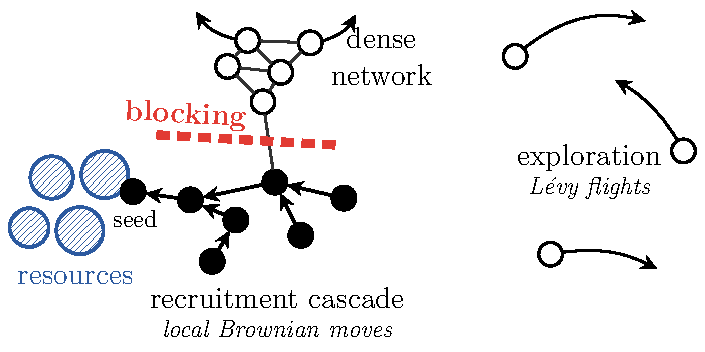
\includegraphics[width=0.86\linewidth]{fig_mechanism_tikz.pdf}
  \caption{\textbf{The physical model.} Agents explore by L\'evy flights (left). An agent that lands on a
  resource---a \emph{seed}---triggers a recruitment cascade along the proximity network, drawing neighbours
  into local convergence on the find; as the neighbourhood crowds, degree-normalized activation $a/k$ falls
  below threshold $\phi$ and further recruitment is \emph{blocked} (red). Reproduced from the companion
  paper~\citep{partI}, where the full model is developed.}
  \label{fig:mech}
\end{figure}

\paragraph{The cascade cycle is an explore/exploit balancer.} The mechanism runs a drive--avalanche cycle
(Fig.~\ref{fig:cycle}): discovery seeds a cascade (explore\,$\to$\,recruit\,$\to$\,exploit), crowding stifles
and disperses it (exploit\,$\to$\,released\,$\to$\,explore), and the swarm self-organizes to a poised operating
point---a ``cascade window'' in connectivity---without any parameter being tuned~\citep{partI}. The companion
paper maps this window with parameter sweeps (phase diagrams over connectivity and activation threshold): the
window's lower edge is the percolation onset and its upper edge is the degree-dependent blocking bound, and
the swarm self-tunes between them. The density-dependent dispersal (``blocking'') is thus what regulates the
explore/exploit \emph{balance}---how much of the swarm explores versus exploits---across the parameter space.
At any instant part of the swarm is exploring and part is exploiting; the cycle continually re-apportions the
two. This is the explore/exploit trade-off being managed, in real time, by the physics rather than by a
controller. A second
fact from the companion paper is load-bearing for the comparisons below and is a consequence of the mechanism,
not a tuning: recruitment is \emph{movement-neutral}---recruited agents reuse the exploring step length and
change only direction, so no movement budget is spent to coordinate~\citep{partI}.

\begin{figure}[t]\centering
  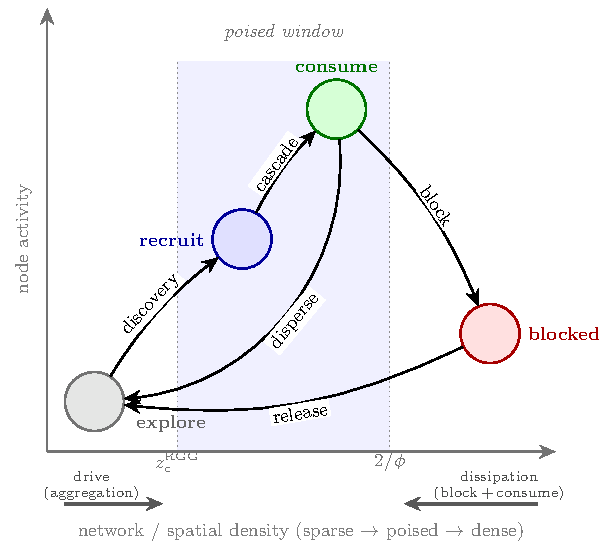
\includegraphics[width=0.62\linewidth]{fig_cycle_schematic_tikz.pdf}
  \caption{\textbf{The self-organizing cycle balances exploration and exploitation.} In the plane of
  network/spatial density (horizontal) and node activity (vertical), the swarm runs a drive--avalanche cycle:
  discovery seeds a recruitment cascade (explore$\to$recruit$\to$exploit); crowding blocks and disperses it
  (exploit$\to$released$\to$explore); aggregation (\emph{drive}) versus dispersal (\emph{dissipation}) hold the
  swarm in a poised window, with no parameter tuned. Reproduced from the companion paper~\citep{partI}.}
  \label{fig:cycle}
\end{figure}

% =====================================================================
\section{The swarm approaches the explore/exploit optimum}
\label{sec:solve}
\paragraph{The problem and its optimum.} Coarse-grain the swarm by the fraction $n_i$ of agents committed to
patch $i$ (the rest exploring); $\mathbf n$ is the swarm's allocation over patches. With resource $Q_i$ shared
among the $N n_i$ foragers working patch $i$, per-capita intake is $f_i=Q_i/(N n_i)$, which falls as a patch
crowds. The optimal allocation---where no forager can raise its intake by moving---equalises per-capita intake
across occupied patches, giving $n_i\propto Q_i$: the ideal free distribution, and the Nash equilibrium of the
habitat-sharing game~\citep{fretwell1969ideal,rosenthal1973congestion} (App.~\ref{app:optimum}). This is the
optimum of the swarm's multi-agent explore/exploit problem: the allocation at which every forager is at its
best available payoff. Because resource is shared, total intake $\sum_i n_i f_i=\sum_i Q_i/N$ is the same for
any interior allocation (App.~\ref{app:optimum}), so this optimum is a load-balancing \emph{equilibrium}, not a
total-harvest maximum; the harvesting-efficiency side of foraging---that finding and exploiting resources
quickly collects more over time---is the companion paper's result~\citep{partI}.

\paragraph{The swarm reaches it, and the coupling causes it.} If the swarm settles at the ideal free
distribution, committed foragers per patch should track patch richness with unit slope. In a heterogeneous
field (Pareto patch richness over a ${\sim}40$-fold range---heavy-tailed, sparse, and clustered, as natural
resource fields typically are) the measured slope is $0.94$ ($R^2=0.67$;
Fig.~\ref{fig:ifd}a)---near-ideal, with the mild \emph{undermatching} real foragers universally show. This is
the \emph{shape} of the optimum (foragers in proportion to richness); how far the swarm sits from the
\emph{exact} equilibrium---its exploitability---is a separate question we quantify against a trained learner in
\S\ref{sec:compare}, where it is measurably exploitable, not at the Nash point. The decisive result for the
causal claim is the ablation: \emph{removing the recruitment coupling collapses the slope to $0.08$}
(Fig.~\ref{fig:ifd}b). The allocation shape is not a property of the individual agents---it is produced by
coupling recruitment to movement. (We attribute no finer mechanism to the coupling than this: in
particular we do \emph{not} claim the coupling implements a particular learning update---\S\ref{sec:how}.)

\begin{figure}[t]
  \centering
  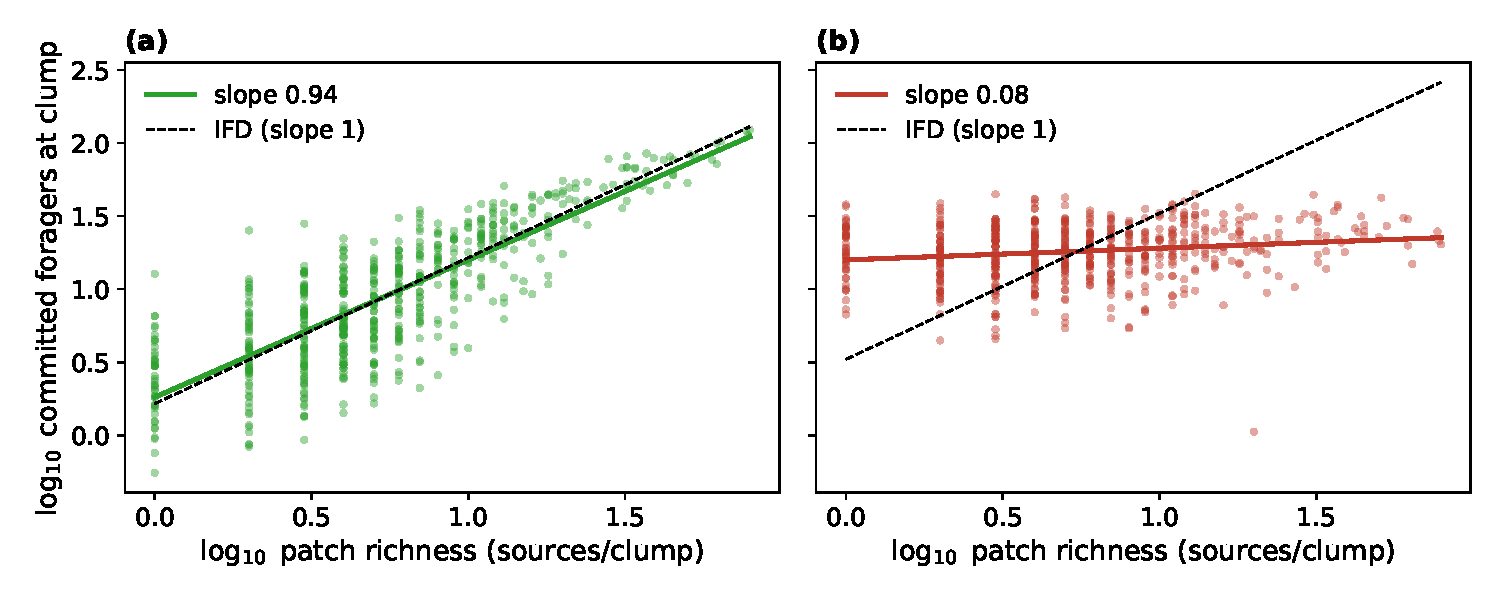
\includegraphics[width=\linewidth]{fig_ifd.pdf}
  \caption{\textbf{The swarm reaches the optimal allocation, and the coupling causes it.} Committed foragers per
  patch vs.\ richness (each point one patch in one run). \textbf{(a) Recruiting.} Slope $0.94$; dashed is the
  ideal slope $1$, the shortfall the ``undermatching'' real foragers show. \textbf{(b) Coupling off.} With
  recruitment removed, matching is destroyed (slope $0.08$): the optimal (ideal-free) allocation is caused by
  the recruitment--movement coupling.}
  \label{fig:ifd}
\end{figure}

\paragraph{The allocation is reached dynamically.} The matching is not imposed; it is \emph{reached}. Tracking
the matching slope through a run (Fig.~\ref{fig:convergence}), the coupled swarm climbs from near zero to its
ideal-free-shape plateau within ${\sim}150$ steps and holds; the uncoupled swarm stays flat. The allocation
is an \emph{attractor} of the explore/exploit dynamics---reached quickly and then maintained.

\begin{figure}[t]\centering
  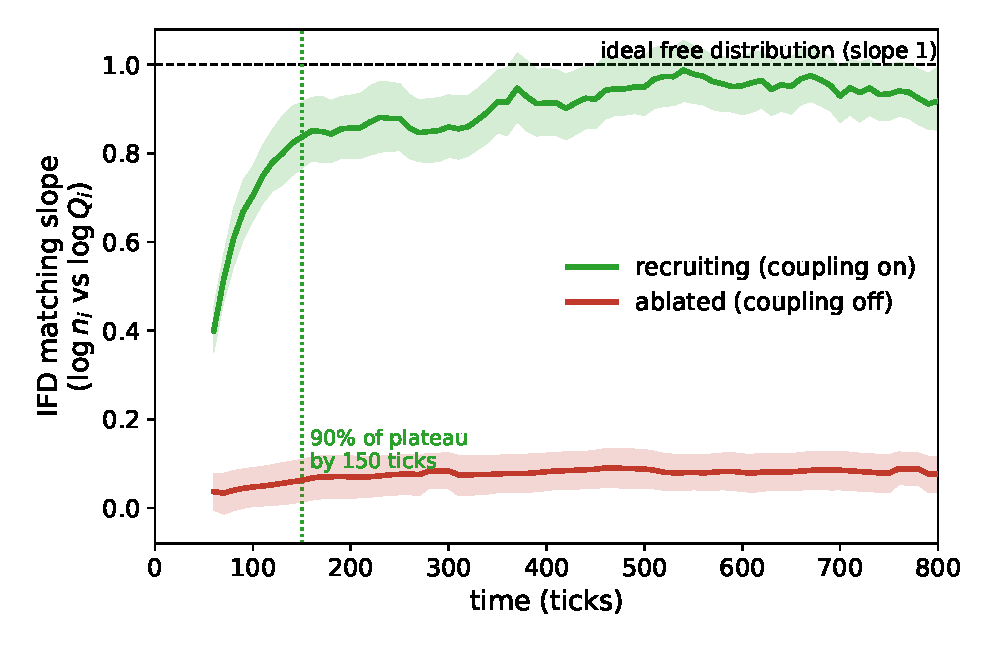
\includegraphics[width=0.72\linewidth]{fig_convergence.pdf}
  \caption{\textbf{The allocation is reached dynamically.} Matching slope (regression of log committed foragers
  per patch on log richness, trailing window; replicas with bootstrap $95\%$ CI) vs.\ time. With the
  recruitment coupling (green) the swarm climbs to the ideal-free plateau (slope $\to1$, dashed) within
  ${\sim}150$ steps and holds; without it (red) matching never develops.}
  \label{fig:convergence}
\end{figure}

\paragraph{The operating regime is self-organized, not tuned.} The swarm is not placed at a hand-chosen
operating point. Sweeping connectivity $\rho_r$ over a $60\times$ density range (Fig.~\ref{fig:selforg}), the
swarm holds a \emph{subcritical} branching ratio $\sigma$ nearly flat ($0.06$--$0.09$)---with its (broad)
minimum near the operating point we use---and maintains near-ideal matching throughout (slope $0.80$--$1.03$),
with no per-condition tuning. We are careful about the sense of ``critical.'' The single-seed recruitment
cascade has the classic window between the percolation onset $z_c^{\mathrm{RGG}}\approx4.51$ and the blocking
bound $2/\phi$ (Fig.~\ref{fig:selforg}a); but because recruited agents aggregate, the swarm's \emph{bulk} mean
degree runs \emph{above} that window, so the criticality is \emph{local} (clusters near-critical, global
branching subcritical), as the companion paper develops~\citep{partI}. What is self-organized here is the
\emph{regime}---a density-invariant subcritical operating point and robust near-ideal matching, reached without
tuning---not a bulk mean degree sitting inside the cascade window.

\begin{figure}[t]\centering
  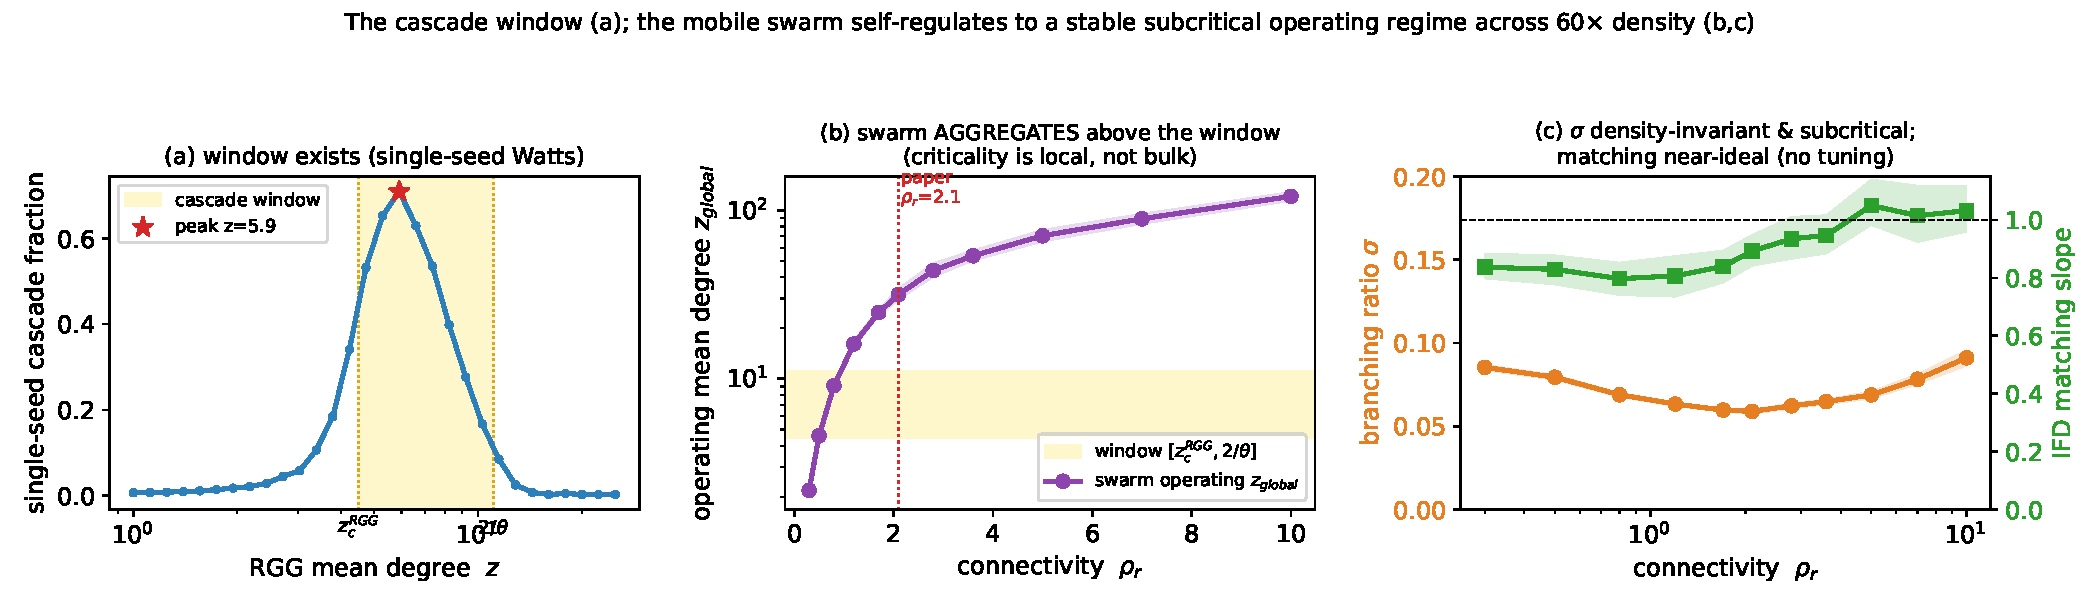
\includegraphics[width=\linewidth]{fig_b1_selforg.pdf}
  \caption{\textbf{The operating regime is self-organized, not tuned.} \textbf{(a)} The single-seed recruitment
  cascade has an inverted-U window between $z_c^{\mathrm{RGG}}\approx4.51$ and the blocking bound $2/\phi$
  (reproduced here). \textbf{(b)} Swept over a $60\times$ connectivity range, the mobile swarm holds a
  subcritical branching ratio $\sigma$ nearly flat ($0.06$--$0.09$), with its broad minimum near the operating
  point used throughout ($\rho_r=2.1$); its bulk mean degree runs \emph{above} the single-seed window (aggregation),
  so the criticality is local, not bulk. \textbf{(c)} Near-ideal IFD matching (slope $0.80$--$1.03$) holds
  across the whole range with no per-condition tuning.}
  \label{fig:selforg}
\end{figure}

% =====================================================================
\section{How it reaches the optimum: learner-free, reward-free, and not by learning}
\label{sec:how}
The swarm reaches the optimum. This section establishes \emph{how it does not}: without a learner, without a
reward signal, and without learning over time. These absences are the content of ``learner-free,'' and we show
each directly rather than asserting it.

\paragraph{No learner.} There are no adjustable parameters and no training phase. Ordinary
RL~\citep{SuttonBarto2018} keeps a value function or a policy network and updates it over many episodes; the
trained parameters are the product. Here the instantaneous configuration $\mathbf n(t)$---carried by the
agents' positions and their interaction network, stored nowhere else---\emph{is} the allocation, taken in real
time, with nothing trained or stored.

\paragraph{No reward signal: recruitment is reward-free by construction.} The decisive evidence is the rule
itself: per-capita intake $f_i$ is never computed or read by any agent---a seed fires on contact with resource,
and recruitment responds to the active \emph{fraction} of neighbours (\S\ref{sec:mech}). There is simply no
reward in the loop, so no reward can be followed; $f_i$ is a quantity \emph{we} compute to describe the
outcome, not a signal the dynamics use. Measurements of the flow are consistent with this but, as we note
below and in App.~\ref{app:dynamics}, cannot by themselves establish it. Illustratively (Fig.~\ref{fig:rewardfree}),
logging per-patch recruitment inflow over $64$ replicas, inflow correlates \emph{positively} with local
occupancy $n_i$ (Pearson $r=+0.11$)---the crowd signal the cascade rule uses---weakly \emph{negatively} with
per-capita payoff $f_i$ ($r=-0.11$), and shows no monotone trend with richness $Q_i$ (non-monotone, linear
$r\approx0$). The negative payoff relation is mechanical: at a patch $n_i f_i=Q_i/N$, so a patch recruitment
has crowded necessarily has low per-capita intake. These correlations are small and illustrative, not an
independent proof of reward-blindness---under equal sharing payoff-rank and distance-from-equilibrium coincide
(App.~\ref{app:dynamics}), so no correlational test can separate ``reward-free'' from ``reward-following.'' The
proof is the construction. The upshot is that the optimum is reached by a mechanism \emph{blind to reward}: the
agents pile onto richer patches only because richer patches, having more resource sites, are discovered and
re-seeded more often, not because anyone measures that they pay better---the strongest sense of ``without a
learner,'' with no reward in the loop to learn from.

\begin{figure}[t]\centering
  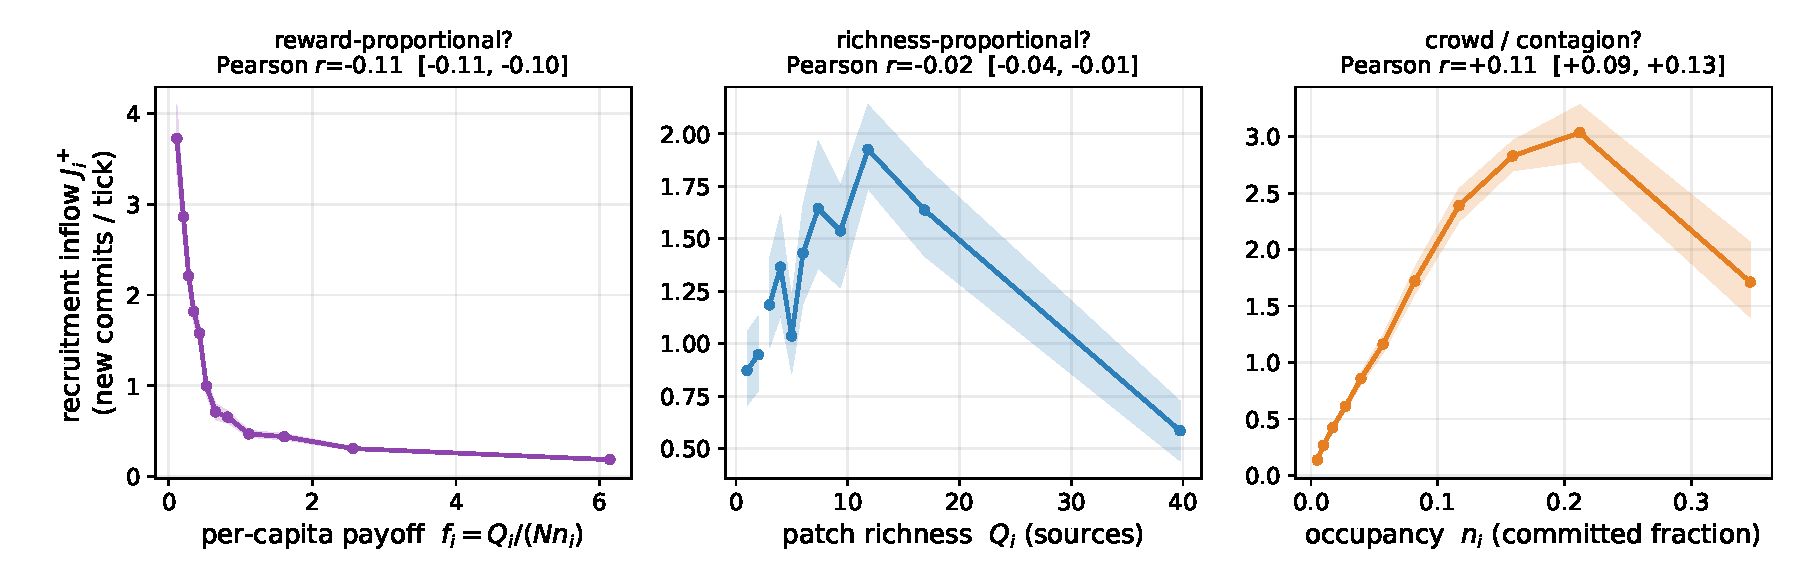
\includegraphics[width=\linewidth]{fig_recruit_vs_payoff.pdf}
  \caption{\textbf{Illustrative: recruitment tracks crowd, not payoff} (reward-freeness itself is established by
  the rule's construction, \S\ref{sec:mech}, not by this figure). Per-patch recruitment inflow $J^+_i$ (new
  commits per step) vs.\ per-capita payoff $f_i$, richness $Q_i$, and occupancy $n_i$ (quantile-binned mean,
  bootstrap $95\%$ CI over $64$ replicas). Inflow correlates positively with occupancy ($r=+0.11$)---the crowd
  signal the cascade rule uses---weakly negatively with payoff ($r=-0.11$), and shows no monotone trend with
  richness (non-monotone, linear $r\approx0$). The correlations are small and, under equal sharing,
  non-identifying (App.~\ref{app:dynamics}); they illustrate rather than prove the reward-free construction.}
  \label{fig:rewardfree}
\end{figure}

\paragraph{What the coarse dynamics are (and are not).} Since the flow carries no reward, is it nonetheless a
reward-following law in disguise? No. Fitting the denoised mean flow of the allocation over the transient to
competing mean-field laws, by leave-replicas-out cross-validation (App.~\ref{app:dynamics}), a
reward-proportional \emph{replicator} update is \emph{not} the best description (held-out $R^2=0.26$); the flow
is a \emph{nonlinear relaxation} toward the ideal-free fixed point (held-out $R^2$ up to $0.64$ for saturating
forms). The coarse dynamics are thus a relaxation of the allocation to the optimum, not a reward-gradient
ascent. We report this as a characterisation of the flow, not as an RL identification: the relaxation reaches
the optimum; it is not a learning update.

\paragraph{It reaches the optimum, it does not learn.} Reaching the optimum is not epistemic learning. The
primary reason is architectural: there is no stored or accumulating state---no value estimate, no counts, no
memory---so there is nothing in which experience could accumulate. Behaviourally this shows as two things
(Fig.~\ref{fig:plateau}): under fixed conditions the allocation's informativeness about the resource field
rises once and \emph{plateaus} by ${\sim}120$ steps rather than improving with more experience; and when the
resources are relocated mid-run, the swarm re-settles to the \emph{same} quality it held before, with no
cumulative gain (relocation at $t{=}400$). (The informativeness metric is bounded, so a plateau alone is only
suggestive; the load-bearing evidence is the absent accumulating state plus the re-tracking to the same, not a
higher, level.) The swarm reaches and \emph{holds} the optimum, re-finding it when the world changes---a
converged, homeostatic policy, not an agent accumulating knowledge.

\begin{figure}[t]\centering
  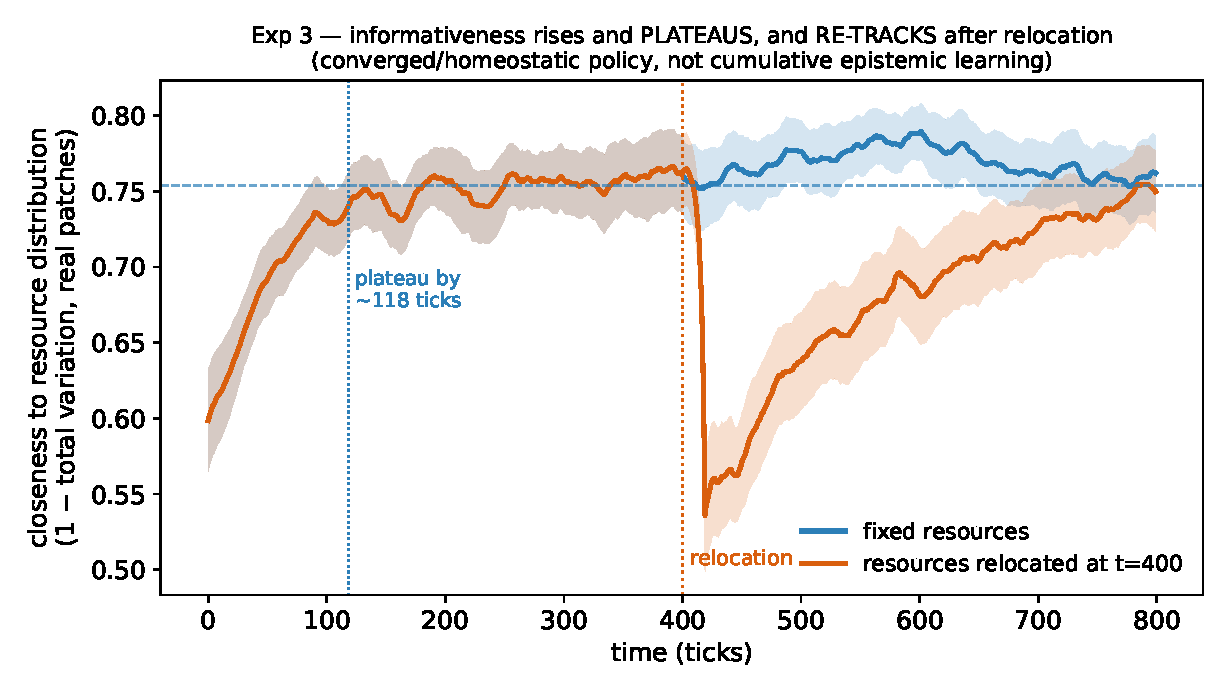
\includegraphics[width=0.74\linewidth]{fig_discrim_plateau.pdf}
  \caption{\textbf{The swarm reaches the optimum but does not learn it.} Allocation informativeness
  (closeness $=1-$ total-variation distance between committed occupancy and the resource distribution; replicas
  with bootstrap $95\%$ CI) vs.\ time. It rises once and \emph{plateaus} by ${\sim}120$ steps; after the
  resources are relocated ($t{=}400$, dashed line) it dips and \emph{re-tracks} to the same plateau, not a
  higher one---no cumulative improvement. This is a converged policy, not a learner.}
  \label{fig:plateau}
\end{figure}

% =====================================================================
\section{Comparison to a trained learner: the verdict depends on embodiment}
\label{sec:compare}
How does a learner-free mechanism compare to an actual learner? We compare in \emph{two} settings, and the
answer flips between them. First, an \emph{abstract} (disembodied) version of the congestion game---direct
patch choice with a per-step payoff oracle and no spatial search---with independent softmax policy-gradient and
$Q$-learning agents (App.~\ref{app:marl}). Second, the \emph{same embodied environment} the swarm acts in: one
spatial world with identical local sensing, movement, and action set $\{$explore, approach, stay$\}$, where the
\emph{only} difference between arms is fixed (recruitment) versus learned (independent per-agent REINFORCE from
local intake) control (App.~\ref{app:embodied}). The first is the comparison a reviewer naturally asks for; the
second is the fair one.

\paragraph{Disembodied, the learner wins on precision.} On the abstract game the swarm reaches the right
allocation \emph{shape} at zero training (matching slope $0.95$---consistent with the $0.94$ in the spatial
field, \S\ref{sec:solve}; $83\%$ of the way to Nash by $1-$ total-variation distance; Fig.~\ref{fig:marl}a) but
is \emph{not} near-optimal on exploitability (Nash-gap $0.58$, roughly $50\times$ a converged $Q$-learner's
$\approx0.011$ and orders of magnitude above a policy-gradient learner's $\approx5\times10^{-4}$;
Fig.~\ref{fig:marl}b). So in this setting a trained learner looks clearly better---it buys precision the swarm
lacks. But the abstract game hands the learner a per-step payoff oracle and removes the spatial search the
swarm must do; the next experiment shows that advantage does not survive matching the problem.

\paragraph{Embodied, the verdict reverses---measured against an oracle ceiling.} In the shared embodied
environment the comparison flips (Fig.~\ref{fig:embodied}). To make the comparison independent of how strong
the learner is, we normalise by a \emph{validated oracle ceiling}: the maximum total intake achievable under
free placement given the current resource state, a strict upper bound (no realised run approaches it). The
reward-free swarm reaches $55\%$ of the ceiling at \emph{zero} training versus the online learner's $34\%$
(equivalently $1.67\times$ the cumulative intake, $65{,}700$ vs $39{,}300$); it also matches the ideal-free
allocation better (slope $0.78$ vs $0.22$) and is far less exploitable (Nash-gap $0.36$ vs $1.34$---the
exploitability ranking \emph{reverses} from the abstract game). (The swarm's own matching is
configuration-specific: slope $0.78$ in this minimal shared environment vs.\ $0.94$ in the richer spatial field
of \S\ref{sec:solve}, so the $0.94$ headline is not universal.) The lead is \emph{robust}: across a $4\times4$
sweep of horizon $T$ and resource-relocation interval (nonstationarity), the swarm leads in \emph{every} cell,
and the margin \emph{grows} with the horizon rather than closing (Fig.~\ref{fig:crossover}). The learner is not
a strawman---its intake converges by ${\sim}100$ steps and it re-adapts after a mid-run relocation, the gap
robust across learning rates ($0.1$--$2.0$)---but it is \emph{architecture-limited, not budget-limited}: it
plateaus at a policy ceiling well below the swarm, and more training does not help. We are careful what this
does and does not show. Both embodied controllers stay well below the ceiling ($23$--$66\%$ swarm, $18$--$34\%$
learner), so the honest reading is that the fixed mechanism is the better \emph{embodied} controller here; that
a \emph{higher-capacity or centralised} learner---not more training---is what it would take to overtake (which
we did not test); and that we therefore claim not that the swarm \emph{beats} reinforcement learning but that
it is \emph{competitive without the learner's overhead} (no training, no reward signal, no parameters), worth
pursuing as a low-overhead coordination primitive. This is one minimal shared environment and one decentralized
learner class, which \emph{bounds} rather than settles the general comparison.

\paragraph{What a learner still buys: transfer.} One advantage of learning is unambiguous. In the abstract
game's non-congestion regime (fixed per-patch reward, optimum $=$ concentrate on the richest patch) the
learners adapt ($80$--$97\%$ of optimum) while the reward-blind swarm keeps spreading and is sub-optimal
($38\%$; Fig.~\ref{fig:marl}c). A learner, by reading reward, transfers across reward structures; the fixed,
reward-blind swarm cannot. (In the embodied environment this regime is not a clean adaptation test---there
intake accrues per agent-on-source, so spreading is near-optimal and the swarm again leads---so we rest the
transfer point on the abstract game.)

\begin{figure}[t]\centering
  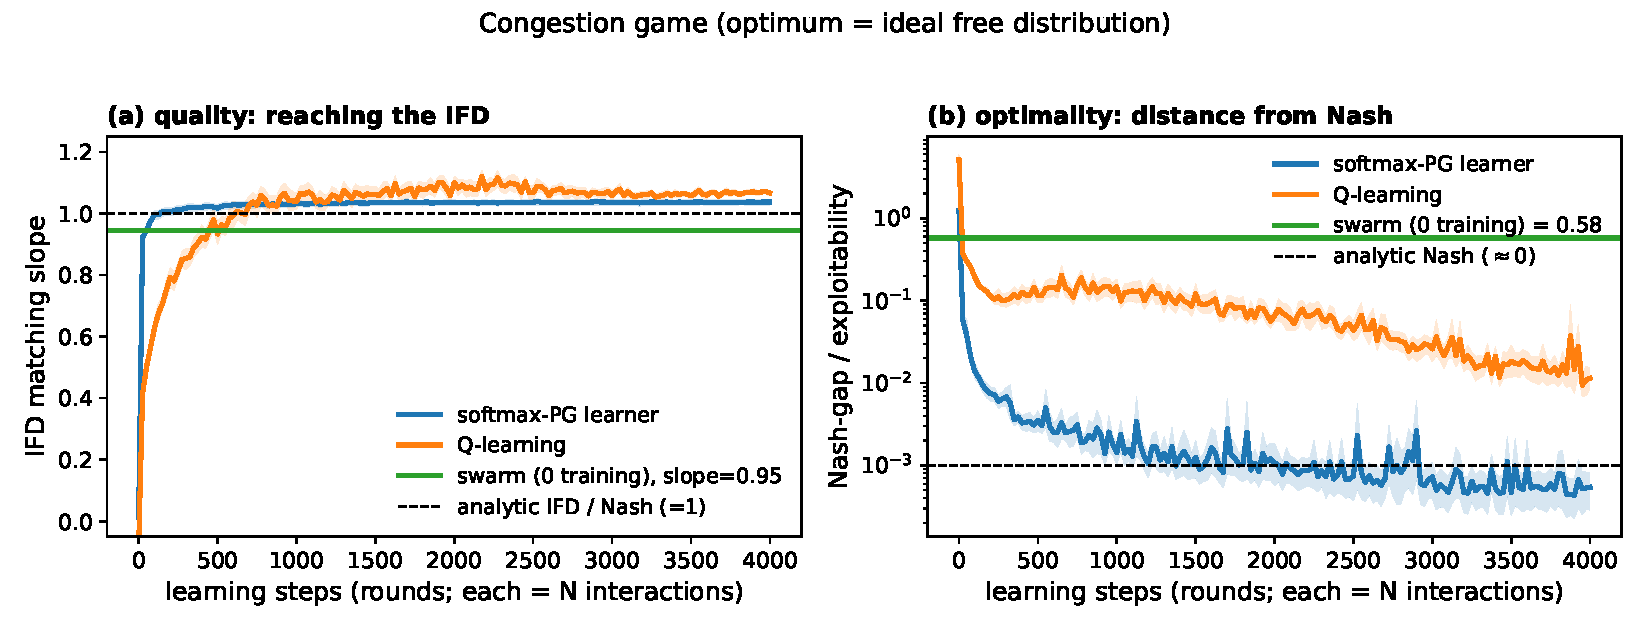
\includegraphics[width=\linewidth]{fig_marl_compare.pdf}\\[5pt]
  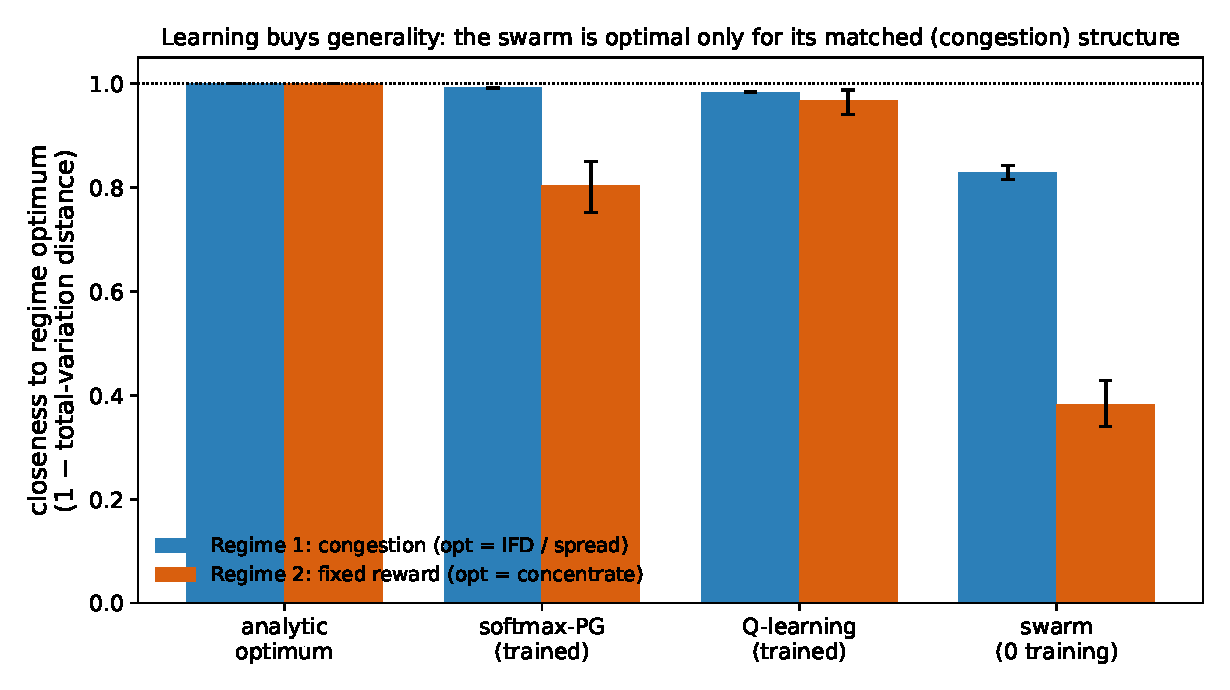
\includegraphics[width=0.66\linewidth]{fig_marl_regimes.pdf}
  \caption{\textbf{Learner-free swarm vs.\ trained multi-agent RL, same optimum (abstract congestion game).}
  \textbf{(a)} matching slope and \textbf{(b)} Nash-gap (exploitability) vs.\ learning steps for independent
  softmax policy-gradient and $Q$-learning (bootstrap $95\%$ CI over $64$ replicas), with the zero-training
  swarm and the analytic optimum as references: the swarm reaches the right allocation \emph{shape} at zero
  training (a), but its Nash-gap ($0.58$) stays well above the trained learners' (b)---it is not near-optimal
  on exploitability. The learners play an easier, disembodied problem (no spatial search); units differ
  (learner steps vs.\ swarm physical steps), as marked. \textbf{(c)} Closeness to the regime optimum in
  the \emph{congestion} regime (optimum $=$ ideal free distribution) and a \emph{non-congestion} regime (fixed
  per-patch reward, optimum $=$ richest patch). The swarm is near-optimal only in the congestion regime its
  mechanism matches; the learners adapt to both. Learning buys generality.}
  \label{fig:marl}
\end{figure}

\begin{figure}[t]\centering
  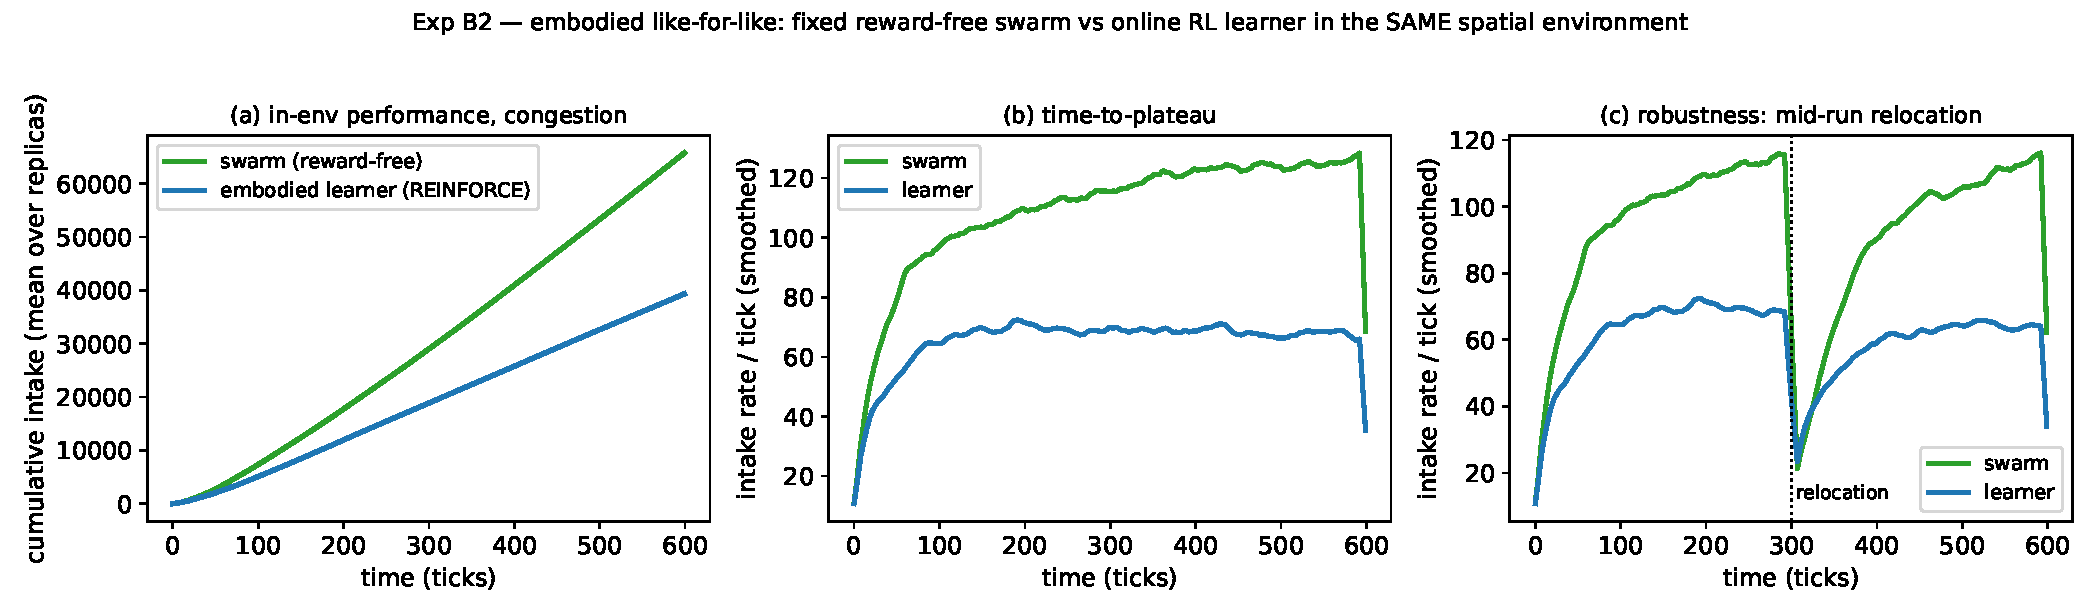
\includegraphics[width=\linewidth]{fig_b2_embodied.pdf}
  \caption{\textbf{Embodied, the reward-free swarm leads the online learner.} Same spatial environment,
  sensing, movement, and action set for both arms; the only difference is fixed (recruitment) vs.\ learned
  (independent per-agent REINFORCE from local intake) control. \textbf{(a)} cumulative intake over the horizon
  (bootstrap $95\%$ CI over $48$ replicas): the swarm collects $1.67\times$ the learner. \textbf{(b)} the
  learner's intake rate converges by ${\sim}100$ steps (not under-trained). \textbf{(c)} after a mid-run
  resource relocation both re-adapt; the swarm recovers faster. The disembodied precision advantage of
  Fig.~\ref{fig:marl} does not survive matching the problem.}
  \label{fig:embodied}
\end{figure}

\begin{figure}[t]\centering
  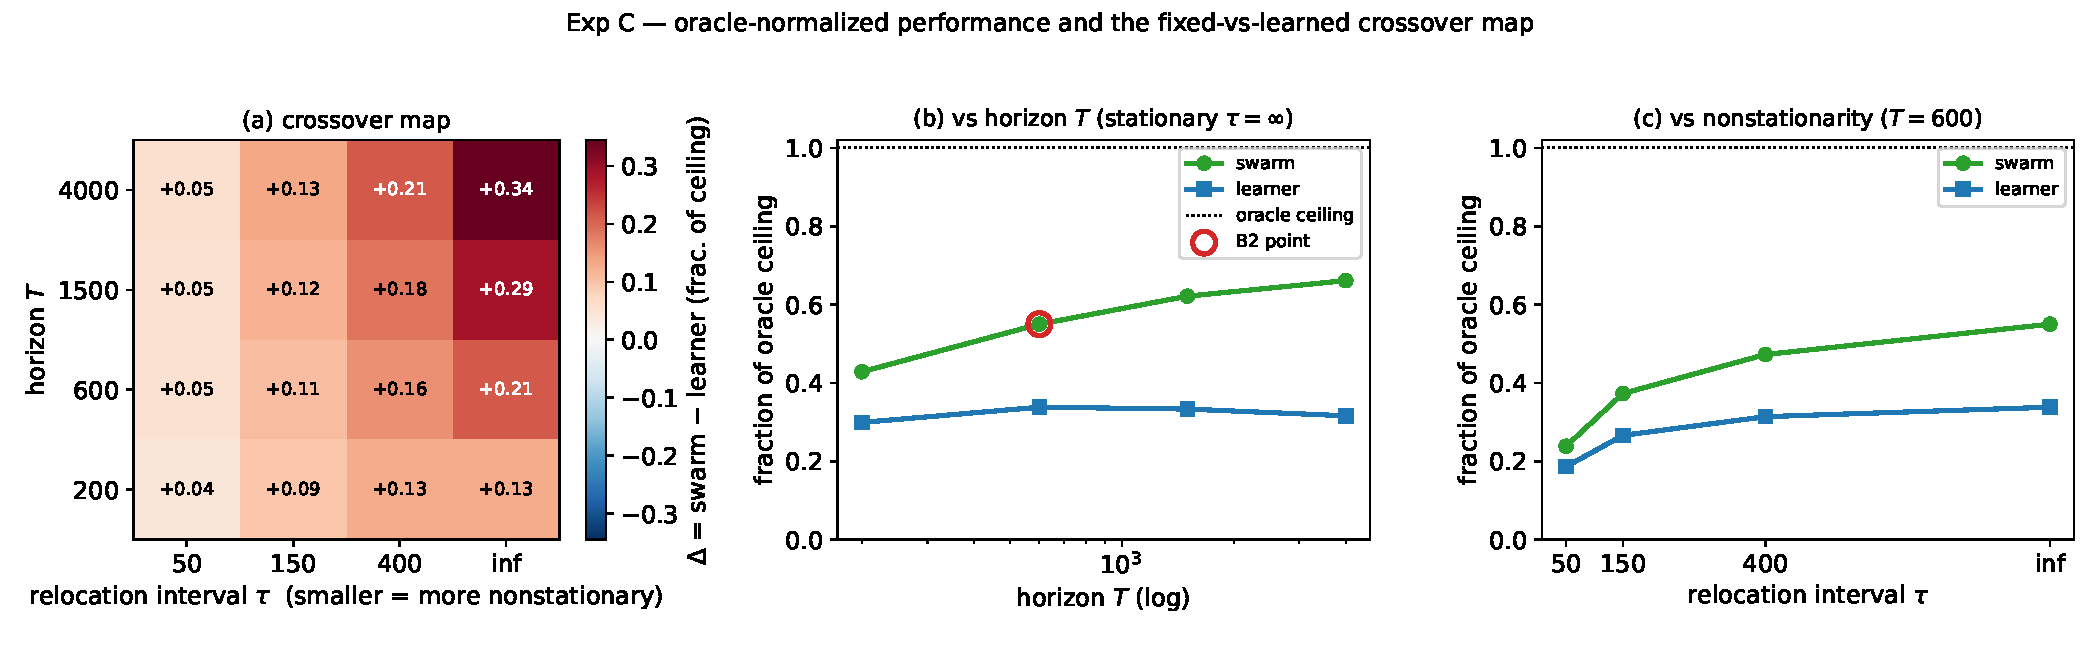
\includegraphics[width=0.82\linewidth]{fig_crossover.pdf}
  \caption{\textbf{The swarm's lead is robust across horizon and nonstationarity.} Fraction of the oracle
  ceiling, swarm minus learner ($\Delta$), over a sweep of horizon $T$ and resource-relocation interval (smaller
  interval $=$ more nonstationary); $B=32$ paired replicas. $\Delta>0$ in all $16$ cells---the swarm is ahead
  everywhere---and the margin \emph{grows} with $T$ (the learner does not amortise; it is architecture-limited)
  and with stationarity. The embodied point of Fig.~\ref{fig:embodied} ($T=600$, stationary) is one cell. Both
  controllers stay well below the ceiling (swarm $23$--$66\%$, learner $18$--$34\%$), so this shows the swarm is
  the better \emph{embodied} controller in this learner class, not that either is near-optimal.}
  \label{fig:crossover}
\end{figure}

\begin{table}[H]
\centering
{\small
\begin{tabular}{@{}p{0.30\linewidth}p{0.32\linewidth}p{0.30\linewidth}@{}}
\hline
\textbf{To reach the optimum} & \textbf{Learner-free swarm (this work)} & \textbf{Trained multi-agent RL} \\
\hline
Reward signal & none (reward-free, Fig.~\ref{fig:rewardfree}) & per-agent scalar payoff, every step \\
Stored parameters & none & $K$ policy values per agent \\
Training before use & none; acts at its operating point & ${\sim}10^3$ update steps \\
Communication & local recruitment only (within range) & none, but needs a reward oracle \\
Movement to coordinate & none beyond exploration (movement-neutral~\citep{partI}) & not embodied (abstract game) \\
Precision, \emph{abstract} game & right shape (slope $0.95$), but exploitable (Nash-gap $0.58$) & near-exact (Nash-gap ${\approx}0$) \\
Exploitability, \emph{embodied} (matched) & \emph{lower}: Nash-gap $0.36$ & higher: Nash-gap $1.34$ \\
Oracle-ceiling fraction, \emph{embodied} (0 training) & $55\%$ of ceiling ($1.67\times$ intake; Fig.~\ref{fig:embodied}) & $34\%$ (after training) \\
Transfer across reward structures & none (congestion/IFD only) & adapts \\
\hline
\end{tabular}}
\caption{\textbf{The two pay for different things.} The learner-free swarm reaches the allocation shape with no
reward signal, no parameters, and no training; the trained learner spends a reward signal, parameters, and
training to buy precision (disembodied) and transfer. The abstract-game learners are disembodied; the fair,
embodied contest (Fig.~\ref{fig:embodied}) is the one where the swarm leads ($1.67\times$ intake), at none of
the learner's overhead. The two Nash-gap rows are different games (abstract vs.\ embodied) and not directly
comparable; the ``movement to coordinate'' row is a companion-paper (supplementary) result, not shown here.}
\label{tab:cost}
\end{table}

% =====================================================================
\section{Discussion}
\paragraph{Where the reinforcement learning is.} The contribution is a demonstration that the \emph{optimum} of
a reinforcement-learning problem---the explore/exploit optimum, here the optimal spatial allocation---can be
\emph{approached} by a self-organizing physical mechanism with none of reinforcement learning's
machinery: the swarm attains the optimum's allocation \emph{shape}, though not its exact equilibrium (it stays
measurably exploitable, \S\ref{sec:compare}). The identification is at the level of the problem and the
allocation reached, not the micro-rule: the dynamics evaluate no reward (by construction) and are not a
reward-following update, and the system reaches this allocation without learning. Read this way, ``learner-free
reinforcement learning'' is a careful statement, not a relabelling: the problem is reinforcement learning's,
the outcome is (approximately) its optimum, and the learner is absent.

\paragraph{Why this is more than aggregation.} A sceptic may ask whether ``reaching the ideal free
distribution'' is just agents piling onto richer patches. Three things make it a genuine optimum rather than a
trivial pile-up. First, the allocation it reaches has the \emph{shape} of the optimum (foragers in proportion
to richness, approaching equal per-capita intake), not an arbitrary aggregation---and the ablation shows it is
non-trivial to reach (without recruitment the swarm does \emph{not} distribute proportionally, slope $0.08$). Second, the explore/exploit trade-off is actively and
continually balanced by the cascade cycle (\S\ref{sec:mech}), not set once. Third, the optimum is an attractor:
the swarm re-finds it when the resources move (Fig.~\ref{fig:plateau}). What it is \emph{not} is a
learner---and we are explicit about that boundary.

\paragraph{Limitations.} (i) The optimum reached is the ideal free distribution of a resource-sharing
(congestion) problem; the swarm's mechanism is matched to that structure and does not transfer to others
(\S\ref{sec:compare}). That structure, however---sparse, patchily clustered resources (heavy-tailed in size and
spacing) shared among foragers---is the common case in natural foraging environments, not a special one, so the
domain the mechanism is matched to is broad and ecologically typical rather than contrived. (ii) Two forces set the allocation, and we separate them. The density-dependent dispersal
(``blocking'') regulates the explore/exploit \emph{balance} and the critical operating point---the companion
paper's parameter sweeps show it bounds the cascade window across connectivity and activation
threshold~\citep{partI}, so the self-organization is load-bearing for the balancing. The allocation
\emph{shape} (slope-one matching), by contrast, is set by richness-proportional discovery and recruitment, not
by the crowding cutoff: a single-operating-point ablation here finds the matching slope essentially unchanged
when the cutoff is removed ($0.94\to0.92$; App.~\ref{app:dynamics}), a consistency check alongside Part I's
swept characterisation. (iii) The
trained-learner comparison includes both an abstract game and an embodied, partially-observed contest
(\S\ref{sec:compare}); the embodied result is one minimal environment with a simple independent learner, so it
\emph{bounds} rather than settles the general swarm-vs-RL question---a richer or centrally-trained learner
could narrow the gap. (iv) We give no closed-form regret or convergence-rate bound.

\paragraph{Outlook.} The crossover sweep (\S\ref{sec:compare}, Fig.~\ref{fig:crossover}) shows the learner's gap
does not close with horizon or nonstationarity---it is architecture-limited---so the decisive open test is a
\emph{higher-capacity} learner (richer observations, a centralised critic): does the swarm's advantage persist
as learner capacity grows? A convergence-rate / regret characterisation of the physical flow against standard
bandit algorithms would also sharpen the reading.

\paragraph{Why it matters.} As an engineering primitive, the mechanism delivers a close approximation of the
explore/exploit optimum---a load-balanced, near-ideal-free allocation---with no model, no reward signal, no
training, and no fitted parameters, deployable on minimal agents---and, matched for embodiment, competitive
with (here ahead of) an online decentralized learner at none of that overhead (\S\ref{sec:compare}). It is a
case where the optimisation \emph{is} the physics of a self-organizing collective, not an algorithm run on top
of it.

% =====================================================================
\section{Conclusion}
A foraging swarm faces the explore/exploit problem that defines reinforcement learning. We have shown that a
minimal self-organizing swarm \emph{approaches its optimum}---balancing exploration and exploitation
through its cascade cycle and converging to the \emph{shape} of the optimal allocation of foragers over patches
(the ideal free distribution)---with no learner, no trained parameters, and no reward signal in its dynamics,
and that it does so by \emph{reaching} this allocation rather than by \emph{learning} it. A trained learner
reaches the optimum more precisely and, unlike the swarm, transfers to other reward structures---the price and
the point of having no learner. The reinforcement learning here is the problem and the (approximate) optimum
reached, emergent from physics.

% =====================================================================
\section*{Competing interests}
Omitted for anonymized review; competing interests are declared in the submission metadata and will be stated
in the camera-ready version.

\section*{Data and code availability}
Complete simulation code, precomputed sweep data, and figure-regenerating scripts are publicly available; the
repository URL is withheld here for anonymized review and will be included in the camera-ready version.

% =====================================================================
\appendix
\section{The optimal allocation: ideal free distribution and habitat-game Nash}
\label{app:optimum}
With resource $Q_i$ shared among the $N n_i$ foragers on patch $i$, per-capita intake is $f_i=Q_i/(N n_i)$.
An allocation is stable against unilateral relocation when per-capita intake is equal across all occupied
patches, $f_i=\bar f$ for all occupied $i$. With $f_i=Q_i/(N n_i)$ this gives $n_i\propto Q_i$: the ideal free
distribution~\citep{fretwell1969ideal}. Because each agent's payoff depends only on how many share its patch,
the habitat-selection game is an anonymous congestion game, whose pure Nash equilibrium is exactly this
equal-intake allocation~\citep{rosenthal1973congestion,wardrop1952road}; player-specific congestion games need
not share this structure~\citep{milchtaich1996congestion}. Note that mean per-capita intake
$\langle f\rangle=\sum_i n_i f_i=\sum_i Q_i/N$ is constant on the interior, so the optimum is an equal-intake
\emph{equilibrium} (a proportional-fair, log-utility allocation~\citep{kelly1998rate}), not a total-intake
maximum: the swarm load-balances, it does not increase total intake. We use the ideal free distribution purely
to \emph{characterise} the solution the swarm reaches (slope-one matching, $n_i\propto Q_i$); the swarm does not
compute payoffs or solve the game (\S\ref{sec:how}).

\section{What the coarse dynamics are: model competition and the role of blocking}
\label{app:dynamics}
\paragraph{Model competition.} We ask which mean-field law best describes the measured flow of the allocation
$\dot n_i$. Per-step $\dot n_i$ is dominated by discrete-event noise (all candidate laws sit at held-out
$R^2\approx0.03$ at step resolution), so we fit the \emph{denoised mean flow}: samples binned by
(richness stratum $\times$ occupancy), each model fit to the per-bin mean $\dot n_i$ over the transient
(steps $1$--$150$), with model selection by leave-$16$-replicas-out cross-validation and AIC/BIC. Candidates:
a reward-proportional \emph{replicator} $\dot n_i=\lambda\,n_i(f_i-\bar f)$ (which on equal sharing is
algebraically a \emph{linear relaxation} to the fixed point, $\lambda'(n_i^*-n_i)$, $n_i^*=Q_i/\sum_jQ_j$);
a saturating \emph{best-response}/logit $\dot n_i=\kappa(\sigma_\beta(f)_i-n_i)$; a payoff-blind
\emph{logistic/contagion} $\dot n_i=\alpha\,n_i(cQ_i-n_i)$; and a constant null. Held-out $R^2$: logit
$0.64$, contagion $0.47$, replicator/linear-relaxation $0.26$, null $0$. Two honest conclusions follow. (i) The
linear replicator/relaxation form is \emph{rejected} as sufficient---the flow has saturating curvature. (ii)
The best-fitting forms are nonlinear \emph{relaxations} toward the $n_i\propto Q_i$ fixed point; because on
equal sharing payoff-rank equals gap-rank, the logit fit does not indicate that the swarm computes payoffs (it
cannot---\S\ref{sec:how}). The flow is a nonlinear relaxation of the allocation to the optimum, consistent with
a reward-free mechanism. Two caveats keep this honest. First, under equal sharing the replicator regressor
$n_i(f_i-\bar f)$ equals the signed distance to the fixed point, $(Q_{\rm tot}/N)(n_i^*-n_i)$ (measured
correlation $0.997$), so payoff-rank and gap-rank coincide and \emph{no} regression on this data can separate a
reward-free from a reward-following rule---reward-freeness rests on the rule's construction (\S\ref{sec:mech}),
not on these fits. Second, the payoff-blind logistic/contagion form, though competitive in bulk $R^2$, is
itself rejected by a shape diagnostic: at small occupancy the measured flow grows with the gap rather than
being throttled toward zero as $n_i(cQ_i-n_i)$ would require. So the fits identify ``nonlinear relaxation to
the fixed point'' but neither a specific reward-following law nor a specific payoff-blind one.

\paragraph{The role of density-dependent dispersal (blocking).} We separate blocking's two possible roles:
setting the explore/exploit \emph{balance} versus setting the allocation \emph{shape}. For the balance,
blocking is causal, and the companion paper establishes this properly with parameter sweeps: its phase diagrams
over connectivity and activation threshold bound the cascade window (percolation onset below, degree-dependent
blocking above), and the swarm self-tunes between them~\citep{partI}. For the allocation shape, we run a single
intermediate ablation here: removing the crowding cutoff (replacing the degree-normalized rule $a/k\ge\phi$ with
an absolute-count rule, the maximal no-cutoff limit) while leaving recruitment otherwise intact. The matching
slope is essentially unchanged ($0.94\to0.92$, no over-aggregation), while the active fraction rises
($0.73\to0.85$)---so blocking was holding more of the swarm exploring (it regulates the balance) but was not
setting the proportional allocation. That shape traces to richness-proportional discovery and recruitment
(richer patches, with more resource sites, are seeded more often). This is a single-operating-point consistency
check, not a sweep---the parameter-dependence of blocking is Part I's result~\citep{partI}, and the
absolute-count toggle is an extreme limit---but together they support attributing the allocation shape to the
recruitment--movement coupling and discovery, while the self-organization (blocking) does the
explore/exploit balancing.

\section{Trained multi-agent RL baseline}
\label{app:marl}
On an abstract version of the congestion allocation game ($K$ patches, $N$ agents, per-capita payoff
$f_i=Q_i/(N n_i)$, richness $Q_i$ matched to the swarm's), each agent runs an independent learner with local,
own-payoff information only: a softmax policy-gradient (REINFORCE with a per-agent baseline) or an
$\epsilon$-greedy $Q$-learner. Quality is the matching slope and the distance to the ideal free distribution;
the ``regret'' analogue is the \emph{exploitability} / Nash-gap, since reward-regret is ill-defined here (mean
per-capita intake is constant, App.~\ref{app:optimum}). The swarm, being reward-blind, is run at its physical
operating point and its steady-state allocation compared on the same $(Q_i,N,K)$. The non-congestion regime
replaces the payoff with a fixed per-patch reward $f_i=Q_i$ (optimum $=$ concentrate on $\arg\max_i Q_i$),
where the swarm's fixed mechanism is sub-optimal while the learners adapt. Learner hyperparameters are lightly
tuned so the baseline is neither crippled nor over-fit; the swarm has no tunable parameters, an asymmetry we
state rather than hide.

\section{Embodied learner comparison}
\label{app:embodied}
Both arms share one spatial environment: a torus with $N=200$ agents, local sensing radius $r$,
Pareto-clumped resources that deplete and respawn, horizon $T=600$. Each agent's observation is local
(on-resource; a resource sensed within range; a binned local fraction of foraging neighbours) and its actions
are $\{$explore (a L\'evy/Brownian step), approach the nearest sensed signal, stay$\}$. The \emph{swarm} arm
applies the fixed recruitment$+$blocking rule over this observation/action set (reward-free); the
\emph{learner} arm replaces the rule with an independent per-agent tabular softmax policy trained online by
REINFORCE with a per-agent baseline, reward $=$ per-capita intake. Only the controller differs---sensing,
movement, and actions are identical---so the comparison isolates fixed versus learned control under matched
embodiment and partial observability. Because both arms use the \emph{same} movement primitives and step
budget, the fairness of this comparison does not rely on the companion paper's movement-neutrality claim: it is
matched by construction here. Metrics are measured in-environment: cumulative intake over the horizon,
IFD matching slope and Nash-gap on the committed occupancy, and recovery after a mid-run resource relocation.
$B=48$ replicas, bootstrap CIs. The learning rate was swept over $\{0.1,0.3,0.6,1.0,2.0\}$ and the gap to the
swarm is robust ($0.52$--$0.62\times$ its intake). This is a deliberately simple, minimal learner, not a tuned
state-of-the-art agent, so the result \emph{bounds} rather than settles the general comparison; the point is
that a fixed reward-free mechanism is not easily matched by \emph{online decentralized} spatial RL under equal
embodiment.

% =====================================================================
\bibliographystyle{tmlr}
\bibliography{refs}

\end{document}
